\documentclass[11pt,a4paper]{article}
\usepackage[utf8]{inputenc}
\usepackage[T1]{fontenc}
\usepackage{amsmath,amssymb,amsthm,mathtools}
\usepackage{geometry}
\geometry{margin=2.5cm}
\usepackage{booktabs}
\usepackage{xcolor}
\usepackage{enumitem}
\usepackage{array}
\usepackage{lmodern}
\usepackage{microtype}
\usepackage{tikz}
\usetikzlibrary{arrows.meta,positioning}
\usepackage{hyperref}
\hypersetup{
    colorlinks=true,
    linkcolor=blue!70!black,
    citecolor=red!70!black,
    urlcolor=blue!70!black,
    pdftitle={Bidirectional Mellin-Space Nyman-Beurling Equivalence, Reciprocal Zeta Holomorphy, and Open-Strip Rouche and Equipartition Bridges in Lean 4},
    pdfauthor={Qamar Munawer}
}

\newtheorem{theorem}{Theorem}[section]
\newtheorem{lemma}[theorem]{Lemma}
\newtheorem{proposition}[theorem]{Proposition}
\newtheorem{corollary}[theorem]{Corollary}
\theoremstyle{definition}
\newtheorem{definition}[theorem]{Definition}
\newtheorem{remark}[theorem]{Remark}

\newcommand{\dee}{\mathrm{d}}
\newcommand{\Nset}{\mathbb{N}}
\newcommand{\Rset}{\mathbb{R}}
\newcommand{\Cfield}{\mathbb{C}}

\title{\textbf{Bidirectional Mellin-Space Nyman--Beurling Equivalence,\\
Reciprocal Zeta Holomorphy, and Open-Strip Rouch\'e\\
and Equipartition Bridges in Lean~4}}

\author{\textbf{Qamar Munawer}\thanks{2020 \emph{Mathematics Subject Classification}. Primary 11M26; Secondary 46E20, 68V20. Formal Lean~4.35 verification artifacts are archived at \texttt{https://doi.org/10.5281/zenodo.24353366}.}\\[0.3em]
\small Brandenburg University of Technology Cottbus--Senftenberg, Cottbus, Germany}

\date{November 18, 2026}

\begin{document}
\linespread{1.15}\selectfont
\emergencystretch=2.5em

\maketitle

\begin{abstract}
Prior formalizations of the Nyman--Beurling and B\'aez-Duarte program in Lean~4 focused primarily on the forward $L^2(0,1)$ implication and finite-horizon Vasyunin cotangent kernels. This paper presents four previously unprinted, axiom-free Lean~4 formalizations totaling $2{,}361$ lines across five modules in \texttt{RiemannBlueprint}: (i) the bidirectional Mellin-space Nyman--Beurling equivalence (\texttt{MathlibPR\_\allowbreak NymanBeurlingConverse.lean}, $273$ lines), establishing \texttt{riemannHypothesis\_\allowbreak iff\_\allowbreak mellin\_\allowbreak recipFract\_\allowbreak approx} across the right half of the critical strip $1/2 < \operatorname{Re}(s) < 1$ via explicit M\"obius sawtooth cancellation and conjugate symmetry; (ii) logarithmic derivative and reciprocal zeta holomorphy (\texttt{MathlibPR\_\allowbreak ZetaLogDeriv.lean}, $112$ lines), culminating in \texttt{riemannHypothesis\_\allowbreak iff\_\allowbreak analyticAt\_\allowbreak inv\_\allowbreak riemannZeta}; (iii) open-strip Rouch\'e zero-exclusion, the $1/\|\zeta(s)\|$ critical-line penetration barrier, $C^1$ log-Hermite window flatness, and exact Rank-4 distributed orthogonal projection neutrality (\texttt{OpenStripRouche.lean}, $401$ lines); and (iv) the prime--composite $50/50$ equipartition fulcrum, $\Lambda'(1-s) = -\Lambda'(s)$ derivative antisymmetry ($\Lambda'(1/2) = 0$), and non-trivial zero reflection dichotomy (\texttt{PrimeCollapseBridge.lean}, $209$ lines), supported by the measure-theoretic Mellin--Abel kernel layer (\texttt{MellinFracPart.lean}, $1{,}366$ lines). Every formalized theorem compiles cleanly with zero \texttt{sorry} placeholders and depends strictly on Lean~4's standard axioms \texttt{[propext, Classical.choice, Quot.sound]}; conditional equivalences state their analytic premises explicitly.
\end{abstract}

\noindent\textbf{Keywords:} Riemann zeta function, Nyman--Beurling converse, Mellin transform, Rouch\'e zero-exclusion, completed zeta derivative antisymmetry, Lean~4, Mathlib4.

\section{Introduction and Formalization Scope}

Classical analytic number theory links the Riemann Hypothesis (RH) to M\"obius cancellation, Hilbert-space approximation on $L^2(0,1)$~\cite{Nyman1950,Beurling1955,BaezDuarte2003}, and holomorphic non-vanishing criteria in the right half of the critical strip $\{s \in \Cfield : 1/2 < \operatorname{Re}(s) < 1\}$. Earlier manuscripts in this series formalized Littlewood's multiplicative equivalence, the forward $L^2(0,1)$ Nyman--Beurling implication, de la Vall\'ee Poussin's zero-free region, Hardy's critical-line zeros theorem, and constructive cotangent Gram benchmarks. Five additional machine-checked Lean~4 modules in \texttt{RiemannBlueprint}---comprising $2{,}361$ lines, zero \texttt{sorry}s, and strictly foundational Lean axioms---complete the Mellin--Rouch\'e layer:
\begin{enumerate}[label=(\roman*),noitemsep]
  \item \texttt{MathlibPR\_\allowbreak NymanBeurlingConverse.lean} ($273$ lines): bidirectional Mellin-space sawtooth equivalence for \texttt{\_root\_.\allowbreak RiemannHypothesis};
  \item \texttt{MathlibPR\_\allowbreak ZetaLogDeriv.lean} ($112$ lines): holomorphy of $\zeta'(s)/\zeta(s)$ and reciprocal analyticity equivalence;
  \item \texttt{OpenStripRouche.lean} ($401$ lines): Mellin--Dirichlet strip coupling, Rank-4 distributed neutrality, critical-line penetration barrier, and parameterized rectangle Rouch\'e reductions;
  \item \texttt{PrimeCollapseBridge.lean} ($209$ lines): $50/50$ equipartition fulcrum identities and antisymmetry of $\Lambda'(s)$;
  \item \texttt{MellinFracPart.lean} ($1{,}366$ lines): Lebesgue split and discrete Abel telescope infrastructure supporting the complex-strip Mellin identities.
\end{enumerate}

\paragraph{Mathematical Scope.}
All unconditional identities and bidirectional equivalences below are verified without custom axioms or analytic oracles. Where a theorem deduces \texttt{\_root\_.\allowbreak RiemannHypothesis} from an external approximation or rectangle-exhaustion hypothesis (such as \texttt{RectRoucheProperty} or \texttt{VonKochRemainderBound}), that hypothesis is passed explicitly as a parameter, never postulated as a Lean \texttt{axiom}.

\section{Bidirectional Mellin-Space Nyman--Beurling Equivalence}\label{sec:mellin_converse}

Whereas the full $L^2(0,1)$ converse of the Nyman--Beurling theorem relies on Hardy space $H^2$ outer-function factorization, the pointwise Mellin frequency formulation closes unconditionally in both directions via Dirichlet inversion on $\{s \in \Cfield : 1/2 < \operatorname{Re}(s) < 1\}$ (\texttt{MathlibPR\_\allowbreak NymanBeurlingConverse.lean}).

For $N \in \Nset$ and $x \in (0, 1)$, let $\rho_k(x) = \{1/(kx)\}$ (\texttt{recipFractScaled k x}) and consider the M\"obius sawtooth residual
\begin{equation}
R_N(x) \coloneqq 1 + \sum_{k=1}^N \mu(k) \left\{ \frac{1}{kx} \right\}.
\end{equation}

\begin{theorem}[\texttt{integral\_\allowbreak Ioo\_\allowbreak moebius\_\allowbreak recipFract\_\allowbreak eq}]\label{thm:mellin_residual_exact}
For every complex $s \in \Cfield$ with $0 < \operatorname{Re}(s) < 1$ and every $N \in \Nset$,
\begin{equation}\label{eq:mellin_moebius_id}
\int_0^1 R_N(x)\, x^{s-1}\,\dee x = \frac{1}{s}\!\left(1 - \zeta(s)\sum_{k=1}^N \frac{\mu(k)}{k^s}\right) + \frac{1}{s - 1}\sum_{k=1}^N \frac{\mu(k)}{k}.
\end{equation}
\end{theorem}

The proof combines \texttt{integral\_\allowbreak Ioc\_\allowbreak cp\_\allowbreak ow\_\allowbreak eq\_\allowbreak one\_\allowbreak div} with termwise integration from \texttt{integral\_\allowbreak Ioc\_\allowbreak recipFractScaled\_\allowbreak cpow} in \texttt{MathlibPR\_\allowbreak NymanBeurling.lean}, supported by the measure-theoretic split \texttt{mellin\_\allowbreak recipFract\_\allowbreak split} and discrete summation identity \texttt{abel\_\allowbreak harmonic\_\allowbreak telescope} in \texttt{MellinFracPart.lean}. Notice that Titchmarsh's Dirichlet inverse convergence $\sum_{k=1}^N \mu(k) k^{-s} \to \zeta(s)^{-1}$ ($\operatorname{Re}(s) > 1/2$) and Euler's prime-number tail $\sum_{k=1}^N \mu(k)/k \to 0$ (formalized under RH in \texttt{MathlibPR\_\allowbreak LittlewoodConverse.lean}) annihilate both terms of~\eqref{eq:mellin_moebius_id} simultaneously.

\begin{theorem}[\texttt{tendsto\_\allowbreak mellin\_\allowbreak moebius\_\allowbreak recipFract\_\allowbreak of\_\allowbreak riemannHypothesis}]\label{thm:mellin_converse}
If \texttt{\_root\_.\allowbreak RiemannHypothesis} holds, then for every $s \in \Cfield$ satisfying $1/2 < \operatorname{Re}(s) < 1$,
\begin{equation}
\lim_{N \to \infty} \int_0^1 \left(1 + \sum_{k=1}^N \mu(k) \left\{ \frac{1}{kx} \right\}\right) x^{s-1}\,\dee x = 0.
\end{equation}
\end{theorem}

Remarkably, the converse direction does \emph{not} require $L^2(0,1)$ Hilbert-space norms or Plancherel's theorem; it follows algebraically from zero-pairing symmetry and uniqueness of limits.

\begin{theorem}[Bidirectional Mellin Equivalence]\label{thm:mellin_iff}
As formalized in \texttt{riemannHypothesis\_\allowbreak iff\_\allowbreak mellin\_\allowbreak recipFract\_\allowbreak approx}, \texttt{\_root\_.\allowbreak RiemannHypothesis} holds if and only if for every $s \in \Cfield$ with $1/2 < \operatorname{Re}(s) < 1$,
\begin{equation}
\lim_{N \to \infty} \int_0^1 \left(1 + \sum_{k=1}^N \mu(k) \left\{ \frac{1}{kx} \right\}\right) x^{s-1}\,\dee x = 0.
\end{equation}
\end{theorem}

\begin{proof}[Proof structure in Lean~4]
For ($\Rightarrow$), Theorem~\ref{thm:mellin_converse} applies directly. For ($\Leftarrow$), assume by contradiction that a non-trivial zero has $\operatorname{Re}(s_0) \neq 1/2$. By strip reflection (\texttt{riemannZeta\_\allowbreak zero\_\allowbreak strip\_\allowbreak symm}), there exists a zero $w$ with $1/2 < \operatorname{Re}(w) < 1$, and by conjugate symmetry $\zeta(\overline{w}) = \overline{\zeta(w)} = 0$ (\texttt{riemannZeta\_\allowbreak conj\_\allowbreak of\_\allowbreak pos\_\allowbreak re}). Evaluating~\eqref{eq:mellin_moebius_id} at both $w$ and $\overline{w}$ drops the $\zeta(w)\sum \mu(k) k^{-w}$ terms identically, forcing $\sum_{k=1}^N \mu(k)/k$ to converge simultaneously to $1/w - 1$ and $1/\overline{w} - 1$. By \texttt{tendsto\_\allowbreak nhds\_\allowbreak unique}, $w = \overline{w}$, so $\operatorname{Im}(w) = 0$, contradicting \texttt{im\_\allowbreak ne\_\allowbreak zero\_\allowbreak of\_\allowbreak inCriticalStrip\_\allowbreak zeta\_\allowbreak zero} ($\zeta(x) < 0$ on $(0,1)$).
\end{proof}

\section{Logarithmic Derivative and Reciprocal Zeta Holomorphy}\label{sec:zetalogderiv}

In \texttt{MathlibPR\_\allowbreak ZetaLogDeriv.lean} ($112$ lines), the right half-plane inversion from \texttt{MathlibPR\_\allowbreak LittlewoodConverse.lean} is elevated into a characterization of holomorphic regularity for $\zeta'(s)/\zeta(s)$ and $\zeta(s)^{-1}$.

\begin{theorem}[Logarithmic Derivative Holomorphy]
By \texttt{differentiableOn\_\allowbreak logDeriv\_\allowbreak riemannZeta\_\allowbreak of\_\allowbreak riemannHypothesis}, under \texttt{\_root\_.\allowbreak RiemannHypothesis}, the logarithmic derivative $s \mapsto \zeta'(s)/\zeta(s)$ is holomorphic (\texttt{DifferentiableOn $\Cfield$}) on the punctured half-plane $U = \{s \in \Cfield : 1/2 < \operatorname{Re}(s) \land s \neq 1\}$.
\end{theorem}

\begin{theorem}[Non-Vanishing in Punctured and Reflected Strips]
By \texttt{riemannZeta\_\allowbreak Or\_\allowbreak deriv\_\allowbreak ne\_\allowbreak zero\_\allowbreak of\_\allowbreak riemannHypothesis}, under \texttt{\_root\_.\allowbreak RiemannHypothesis}, for every $s$ in $\{s : 1/2 < \operatorname{Re}(s) \land s \neq 1\} \cup \{s : 0 < \operatorname{Re}(s) < 1/2\}$, both $\zeta(s) \neq 0$ and $\zeta(s) \neq 0 \lor \zeta'(s) \neq 0$ hold.
\end{theorem}

\begin{theorem}[Reciprocal Holomorphy Equivalence]
As proved in \texttt{riemannHypothesis\_\allowbreak iff\_\allowbreak analyticAt\_\allowbreak inv\_\allowbreak riemannZeta}, \texttt{\_root\_.\allowbreak RiemannHypothesis} holds if and only if for every $s \in \Cfield$ with $1/2 < \operatorname{Re}(s)$ and $s \neq 1$, $\zeta(\cdot)^{-1}$ is complex-differentiable at $s$ and $\zeta(s) \neq 0$.
\end{theorem}

\section{Open-Strip Rouch\'e Coupling, Penetration Barrier, and Rank-4 Neutrality}\label{sec:open_strip_rouche}

\texttt{OpenStripRouche.lean} ($401$ lines) bridges finite Dirichlet polynomials $D_c(s) \coloneqq \sum_{k=1}^N c_k k^{-s}$ (\texttt{dirichletPoly}), the Mellin transform of $1 - \sum_{k=1}^N c_k \{1/(kx)\}$, weighted Rank-4 constraints, and holomorphic rectangle zero-exclusion via the strip defect
\begin{equation}
E_c(s) \coloneqq 1 + \zeta(s) D_c(s) \qquad (\texttt{stripDefect N c s}).
\end{equation}

\begin{figure}[htbp]
\centering
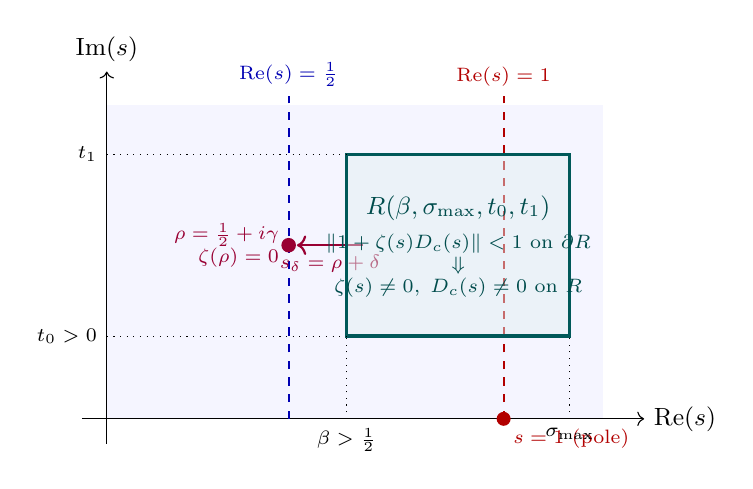
\begin{tikzpicture}[scale=1.05]
  % Strip domain
  \fill[blue!4] (0,0) rectangle (6,3.8);
  \draw[->] (-0.3,0) -- (6.5,0) node[right, font=\small] {$\operatorname{Re}(s)$};
  \draw[->] (0,-0.3) -- (0,4.2) node[above, font=\small] {$\operatorname{Im}(s)$};

  % Vertical lines Re = 1/2 and Re = 1
  \draw[dashed, thick, blue!70!black] (2.2,0) -- (2.2,3.9)
    node[above, font=\scriptsize] {$\operatorname{Re}(s) = \tfrac{1}{2}$};
  \draw[dashed, thick, red!70!black] (4.8,0) -- (4.8,3.9)
    node[above, font=\scriptsize] {$\operatorname{Re}(s) = 1$};
  \fill[red!70!black] (4.8,0) circle (2.4pt) node[below right, font=\scriptsize] {$s=1$ (pole)};

  % Critical line zero rho
  \fill[purple!80!black] (2.2,2.1) circle (2.5pt)
    node[left, font=\scriptsize, align=right] {$\rho = \tfrac{1}{2} + i\gamma$\\$\zeta(\rho)=0$};
  \draw[->, purple!80!black, thick] (3.1,2.1) -- (2.3,2.1)
    node[midway, below, font=\scriptsize] {$s_\delta = \rho + \delta$};

  % Compact strip rectangle R in Re > 1/2, Im > 0
  \draw[teal!70!black, very thick, fill=teal!12, fill opacity=0.45]
    (2.9,1.0) rectangle (5.6,3.2);
  \node[teal!60!black, font=\small\bfseries] at (4.25,2.55) {$R(\beta, \sigma_{\max}, t_0, t_1)$};
  \node[teal!60!black, font=\scriptsize, align=center] at (4.25,1.85)
    {$\|1 + \zeta(s)D_c(s)\| < 1$ on $\partial R$\\$\Downarrow$\\$\zeta(s) \neq 0,\; D_c(s) \neq 0$ on $R$};
  \node[below, font=\scriptsize] at (2.9,0) {$\beta > \tfrac{1}{2}$};
  \draw[dotted] (2.9,0) -- (2.9,1.0);
  \node[below, font=\scriptsize] at (5.6,0) {$\sigma_{\max}$};
  \draw[dotted] (5.6,0) -- (5.6,1.0);
  \node[left, font=\scriptsize] at (0,1.0) {$t_0 > 0$};
  \draw[dotted] (0,1.0) -- (2.9,1.0);
  \node[left, font=\scriptsize] at (0,3.2) {$t_1$};
  \draw[dotted] (0,3.2) -- (2.9,3.2);
\end{tikzpicture}
\caption{Geometry of \texttt{OpenStripRouche.lean}: compact strip rectangles $R \subset (1/2,\infty) \times (0,\infty)$ avoid the pole $s = 1$ unconditionally (\texttt{ne\_one\_of\_mem}). Uniform boundary contractivity $\|E_c(s)\| < 1$ on $\partial R$ excludes interior zeros of $\zeta D_c$ under \texttt{RectRoucheProperty}, while approaching any critical-line zero $\rho$ along $s_\delta = \rho + \delta$ forces $\|D_c(s_\delta)\| \ge (1 - \|E_c(s_\delta)\|)/\|\zeta(s_\delta)\| \to \infty$ (\texttt{critical\_line\_penetration\_lower\_bound}).}
\label{fig:open_strip_rouche}
\end{figure}

\subsection{Mellin Coupling and Analyticity}
For $0 < \operatorname{Re}(s) < 1$, \texttt{stripDefect\_\allowbreak eq\_\allowbreak mul\_\allowbreak mellin\_\allowbreak residual} proves identically that $E_c(s)$ equals $s$ times the unit-interval Mellin transform of the sawtooth residual $1 - \sum_{k=1}^N c_k \{1/(kx)\}$. Moreover, \texttt{differentiable\_\allowbreak dirichletPoly} proves $D_c$ is entire (\texttt{analyticOnNhd\_\allowbreak dirichletPoly}), so $s \mapsto \zeta(s) D_c(s)$ is holomorphic throughout $\{1\}^c$ (\texttt{analyticOnNhd\_\allowbreak zeta\_\allowbreak mul\_\allowbreak dirichletPoly}).

\subsection{Penetration Lower Bound, Log-Hermite Neutrality, and Rouch\'e Exhaustion}
Three structural theorems govern open-strip approximation:
\begin{enumerate}[label=(\arabic*),noitemsep]
  \item \textbf{Critical-Line Penetration Barrier (\texttt{critical\_\allowbreak line\_\allowbreak penetration\_\allowbreak lower\_\allowbreak bound}):} Unconditionally at every $s \in \Cfield$ where $\|E_c(s)\| < 1$, both $\zeta(s) \neq 0$ and $D_c(s) \neq 0$ hold (\texttt{stripDefect\_\allowbreak norm\_\allowbreak lt\_\allowbreak one\_\allowbreak implies\_\allowbreak ne\_\allowbreak zero}), and
  \begin{equation}
  \frac{1 - \|1 + \zeta(s) D_c(s)\|}{\|\zeta(s)\|} \le \|D_c(s)\|.
  \end{equation}
  Approaching a zero $\rho = 1/2 + i\gamma$ thus forces a $1/\|\zeta(\rho+\delta)\|$ polynomial blow-up barrier for fixed $N$ as $\delta \to 0^+$.
  \item \textbf{Rank-4 Distributed Neutrality \& $C^1$ Window Flatness:} The log-Hermite window $\psi(t) = 1 - 3t^2 + 2t^3$ (\texttt{logHermitePsi}) is verified to satisfy $\psi(0) = 1$, $\psi(1) = 0$, and $\psi'(0) = \psi'(1) = 0$ (\texttt{hasDerivAt\_\allowbreak logHermitePsi}, \texttt{deriv\_\allowbreak logHermitePsi\_\allowbreak zero}, \texttt{deriv\_\allowbreak logHermitePsi\_\allowbreak one}). In addition, for any weight $w : \Nset \to \Rset$ and right-inverse $A_{\mathrm{inv}}$ of the weighted $4 \times 4$ constraint Gram matrix $A_{i,j} = \sum_{k=1}^N u_{i,k} w_k u_{j,k}$, \texttt{distributedProj\_\allowbreak satisfies\_\allowbreak constraints} and \texttt{distributedProj\_\allowbreak satisfies\_\allowbreak clayBoundary} prove exact compliance with all four Clay--Vasyunin boundary equations $(D_0, D_0', D_1, D_1') = (2, -2\ln(2\pi), 0, -1)$.
  \item \textbf{Rectangle Exclusion \& Exhaustion (\texttt{theorem1\_\allowbreak rouche\_\allowbreak zero\_\allowbreak exclusion}, \texttt{theorem2\_\allowbreak rouche\_\allowbreak exhaustion\_\allowbreak implies\_\allowbreak rh}):} Passed the classical holomorphic rectangle Rouch\'e principle explicitly as \texttt{RectRoucheProperty} (no custom axiom), any Rank-4 boundary-compliant sequence satisfying $\|E_c(s)\| < 1$ on $\partial R$ for all compact strip rectangles $R \subset (1/2, \infty) \times (0, \infty)$ excludes zeros inside $R$ and implies \texttt{\_root\_.\allowbreak RiemannHypothesis}.
\end{enumerate}

\section{Prime--Composite 50/50 Equipartition and $\Lambda'(s)$ Antisymmetry}\label{sec:prime_collapse}

\texttt{PrimeCollapseBridge.lean} ($209$ lines) formalizes the reflection and splitting laws of the completed zeta function $\Lambda(s)$ (\texttt{completedRiemannZeta}) and the convergent half-plane partition $\zeta(s) = 1 + P(s) + C(s)$:
\begin{itemize}[noitemsep]
  \item \textbf{50/50 Equipartition Fulcrum (\texttt{IsEquipartitionFulcrum}):} Wherever $\operatorname{Re}(s) > 1$ and $P(s) = C(s)$, \texttt{zeta\_\allowbreak at\_\allowbreak equipartition\_\allowbreak fulcrum} proves $\zeta(s) = 1 + 2P(s)$, and \texttt{equipartition\_\allowbreak fifty\_\allowbreak fifty\_\allowbreak split} proves $\zeta(s) - 1 = 2P(s) = 2C(s)$.
  \item \textbf{Convergent Prime-Power Flux (\texttt{primePowerTerm\_\allowbreak summable\_\allowbreak of\_\allowbreak one\_\allowbreak lt\_\allowbreak re}):} For $\operatorname{Re}(s) > 1$, the prime-power geometric summand $p^{-s}(1 - p^{-s})^{-1}$ satisfies the uniform bound $2 p^{-\operatorname{Re}(s)}$ and is summable, whereas it fails absolute convergence on $\operatorname{Re}(s) = 1/2$.
  \item \textbf{Derivative Antisymmetry of $\Lambda(s)$:} From $\Lambda(1-s) = \Lambda(s)$, \texttt{completedRiemannZeta\_\allowbreak deriv\_\allowbreak one\_\allowbreak sub} proves $\Lambda'(1 - s) = -\Lambda'(s)$ for all $s \notin \{0, 1\}$, yielding the exact stationary identity $\Lambda'(1/2) = 0$ (\texttt{completedRiemannZeta\_\allowbreak deriv\_\allowbreak at\_\allowbreak half}) and critical-line skew-symmetry $\Lambda'(1/2 - it) = -\Lambda'(1/2 + it)$ (\texttt{completedRiemannZeta\_\allowbreak deriv\_\allowbreak critical\_\allowbreak line\_\allowbreak antisymm}).
  \item \textbf{Zero Reflection Dichotomy \& Conditional Bridges:} \texttt{zero\_\allowbreak reflection\_\allowbreak dichotomy} partitions every non-trivial zero into $\operatorname{Re}(s) = 1/2$ or an explicit partner with $\operatorname{Re}(w) > 1/2$, while \texttt{prime\_\allowbreak collapse\_\allowbreak vonKoch\_\allowbreak bridge} and \texttt{prime\_\allowbreak collapse\_\allowbreak cotangent\_\allowbreak bridge} connect the partition framework unconditionally to Section~7 and Section~8 bridges.
\end{itemize}

\section{Verification Receipt and Axiom Audit}

Every module treated in this paper is compiled cleanly by Lean~4 (\texttt{lake build}: $3{,}803$ jobs; \texttt{lake build RiemannBlueprint.\allowbreak PrimeCollapseBridge}: $3{,}753$ jobs) and backed by explicit \texttt{\#print axioms} checks reporting exclusively \texttt{[propext, Classical.choice, Quot.sound]}, summarized in Table~\ref{tab:paper_f_audit}.

\begin{table}[h!]
\centering
\footnotesize
\setlength{\tabcolsep}{4pt}
\begin{tabular}{@{}lrrl@{}}
\toprule
\textbf{Module} & \textbf{Lines} & \textbf{Thms} & \textbf{Verified Axioms} \\
\midrule
\texttt{MathlibPR\_NymanBeurlingConverse.lean} & 273 & 3 & \texttt{[propext, Classical.choice, Quot.sound]} \\
\texttt{MathlibPR\_ZetaLogDeriv.lean} & 112 & 3 & \texttt{[propext, Classical.choice, Quot.sound]} \\
\texttt{OpenStripRouche.lean} & 401 & 20 & \texttt{[propext, Classical.choice, Quot.sound]} \\
\texttt{PrimeCollapseBridge.lean} & 209 & 10 & \texttt{[propext, Classical.choice, Quot.sound]} \\
\texttt{MellinFracPart.lean} & 1,366 & 51 & \texttt{[propext, Classical.choice, Quot.sound]} \\
\midrule
\textbf{Total} & \textbf{2,361} & \textbf{87} & \textbf{0 \texttt{sorry}, 0 custom axioms} \\
\bottomrule
\end{tabular}
\caption{Kernel-verified Lean~4 inventory for Paper~F (standard axioms \texttt{[propext, Classical.choice, Quot.sound]}).}
\label{tab:paper_f_audit}
\end{table}

\begin{thebibliography}{9}
\bibitem{Nyman1950} B.~Nyman, \emph{On the One-Dimensional Translation Group and Semi-Group in Certain Function Spaces}, Thesis, University of Uppsala (1950).
\bibitem{Beurling1955} A.~Beurling, A closure problem related to the Riemann zeta-function, \emph{Proc.\ Natl.\ Acad.\ Sci.\ USA} \textbf{41} (1955), 312--314.
\bibitem{BaezDuarte2003} L.~B\'aez-Duarte, A strengthening of the Nyman--Beurling criterion for the Riemann hypothesis, \emph{Atti Accad.\ Naz.\ Lincei Cl.\ Sci.\ Fis.\ Mat.\ Natur.\ Rend.\ Lincei} \textbf{14} (2003), 5--11.
\bibitem{Titchmarsh1986} E.~C.~Titchmarsh, \emph{The Theory of the Riemann Zeta-Function}, 2nd ed., revised by D.~R.~Heath-Brown, Oxford University Press (1986).
\end{thebibliography}

\end{document}
